\documentclass[11pt]{beamer}
\usetheme[sectionpage=none,numbering=none]{metropolis}           % Use metropolis theme
	% To do printouts, add ", handout"  after aspectratio.
    % So we make this "beamer" rather than document!
\usepackage{booktabs}
\usepackage{graphicx}
\usepackage{color}

\title{Mass Incarceration and Mandatory Minimums}
\author{Nick Eubank}
\date{\vspace*{.3in} \today}


% This is the beginning of a real document!
\begin{document}

\begin{frame}
	\maketitle
\end{frame}

\begin{frame}[c]{Question}
What is the effect of \alert{mandatory minimum sentences} on \alert{incarceration rates?}\\
\vspace{1cm}
\pause Mandatory minimums: Laws that set (often high) minimum sentences for crimes, \\
\pause rather than make recommendations and let judges / juries determine sentences on a case by case basis.
\end{frame}

\begin{frame}[c]{Motivation}
\begin{figure}
	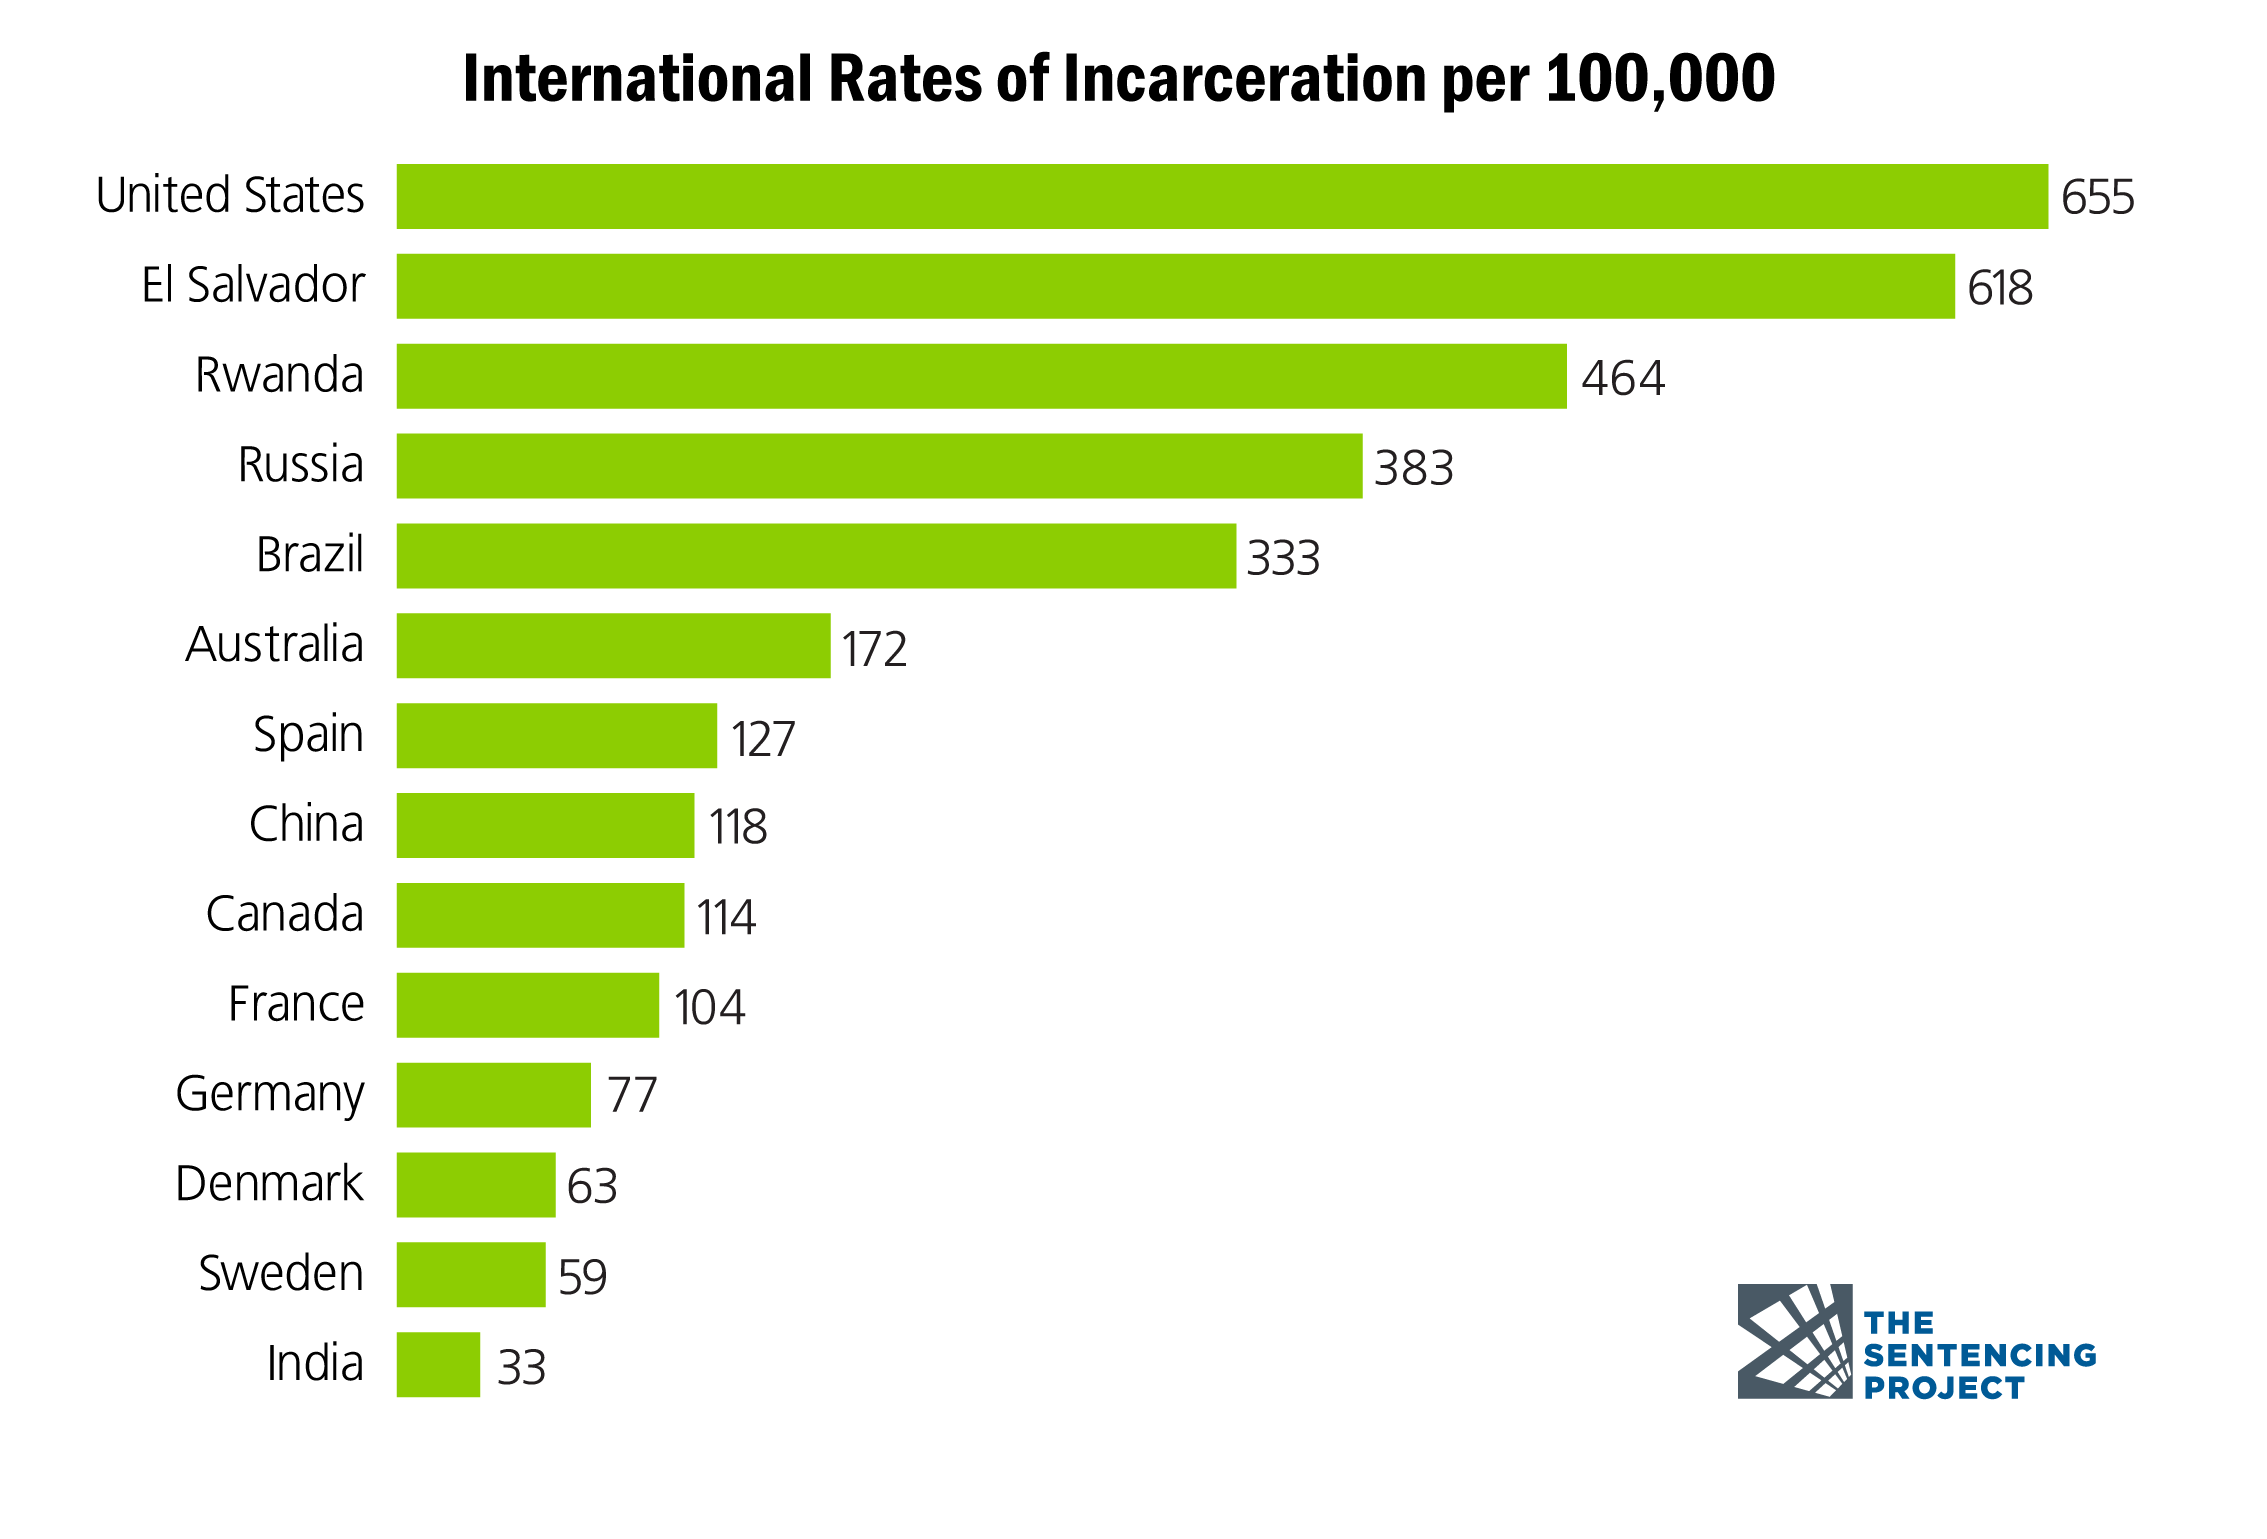
\includegraphics[width=\textwidth]{international_comparison.png}
\end{figure}
\end{frame}

\begin{frame}[c]{Motivation}
\begin{figure}
	\pause 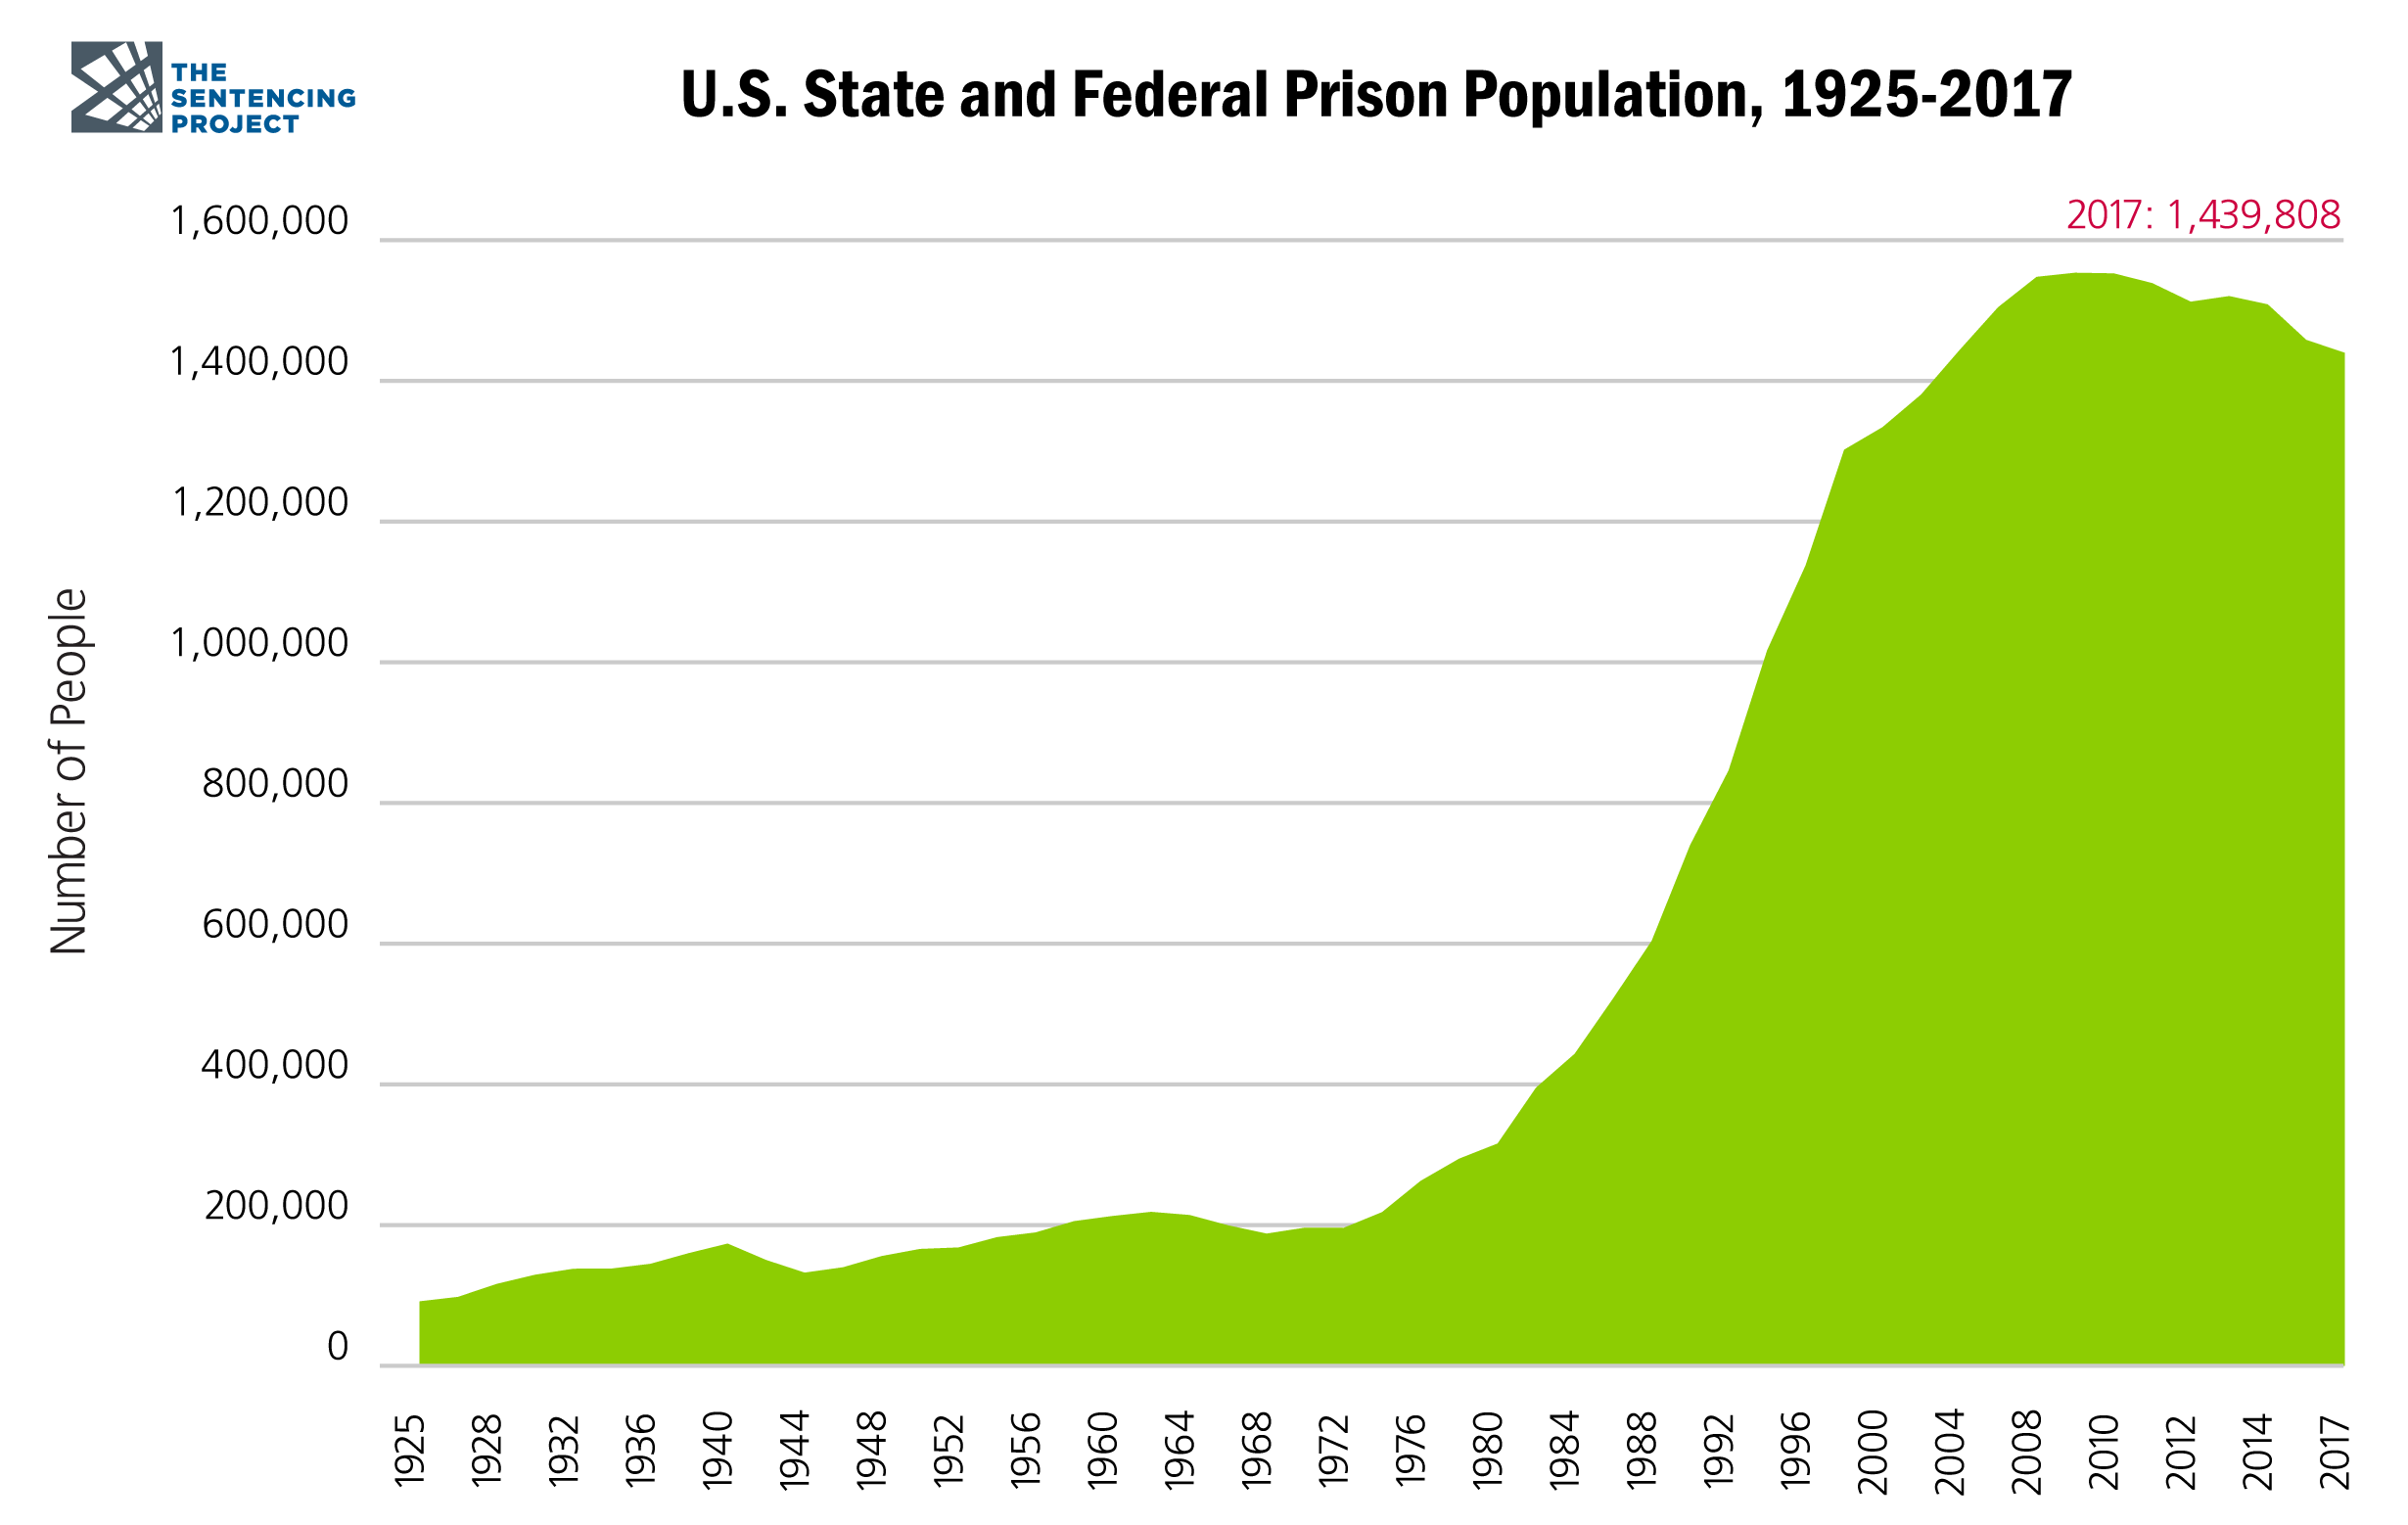
\includegraphics[width=\textwidth]{incarceration_trends.png}
\end{figure}
\end{frame}


\begin{frame}[c]{Mandatory Minimums?}
Starting in the mid-1980s, US States began passing new mandatory minimum legislation.
\begin{itemize}
    \pause \item Dramatically increased minimum sentences for crimes.
\end{itemize}
\pause California three strikes:
\begin{itemize}
    \item If convinced of three felonies in your life, sentence for third was 25-to-life, regardless of crime.
\end{itemize}
\pause 25-to-life for burglary.\\
\pause \vspace{1cm}
Did this $\leadsto$ $\uparrow$ incarceration?
\end{frame}

\begin{frame}[c]{Mandatory Minimums?}
Very few criminals actually serving ``mandatory minimum'' sentences.
\begin{itemize}
    \item {\color{gray} Pfaff (2017)}
\end{itemize}
\pause So how could they be to blame?
\end{frame}

\begin{frame}[c]{Mandatory Minimums?}
In the US, $> 95\%$ of criminal cases are resolved using plea bargains. \\
\vspace{1cm}
\pause Maybe the ability of prosecutors to \alert{threaten} defendants with a crime that carries a large minimum sentence $\leadsto$ defendants pleading guilty to lesser crimes.
\end{frame}

\begin{frame}[c]{Question}
    Does the passage of \alert{mandatory minimum legislation} make defendants:
    \begin{enumerate}
        \item More likely to plead guilty to a crime
        \item More likely to plead guilty to more serious crimes / accept longer sentences.
    \end{enumerate}
\end{frame}


\begin{frame}[c]{Ideal Experiment}
\begin{itemize}
    \item Randomly assign defendants to \alert{potentially} face mandatory minimums
    \pause \item Observe resulting plea bargains
\end{itemize}
\pause Test:
\begin{itemize}
    \item Do defendants under \alert{threat} of mandatory minimums accept more punitive deals.
\end{itemize}
\end{frame}


\begin{frame}[c]{Feasible Design \#1}
California passed mandatory minimum legislation in 1994\\
\pause
\vspace{1cm}
Difference in Difference Design:
\begin{itemize}
    \item Difference 1: Pre-to-post 1994
    \item Difference 2: Whether state has passed mandatory minimum legislation (e.g. California versus non-California).
\end{itemize}
\pause Sample:
\begin{itemize}
    \item Western US states: Oregon, Nevada, Arizona.
    \item Exclude Washington because also had changes in mandatory minimums in 1995.
\end{itemize}
\pause
Control for crime rates
\end{frame}


\begin{frame}[c]{Assumptions of Design \#1}
Absent changes in mandatory minimums, incarceration rates in Western US states would have had parallel trajectories.
\begin{itemize}
    \item \emph{Empirically Testable}
\end{itemize}
\pause (If control for crime rates: need parallel trends \emph{after} controlling for crime rates).
\end{frame}

\begin{frame}[c]{}

\begin{figure}
    \centering
    \caption{If Increase Incarceration}\label{}
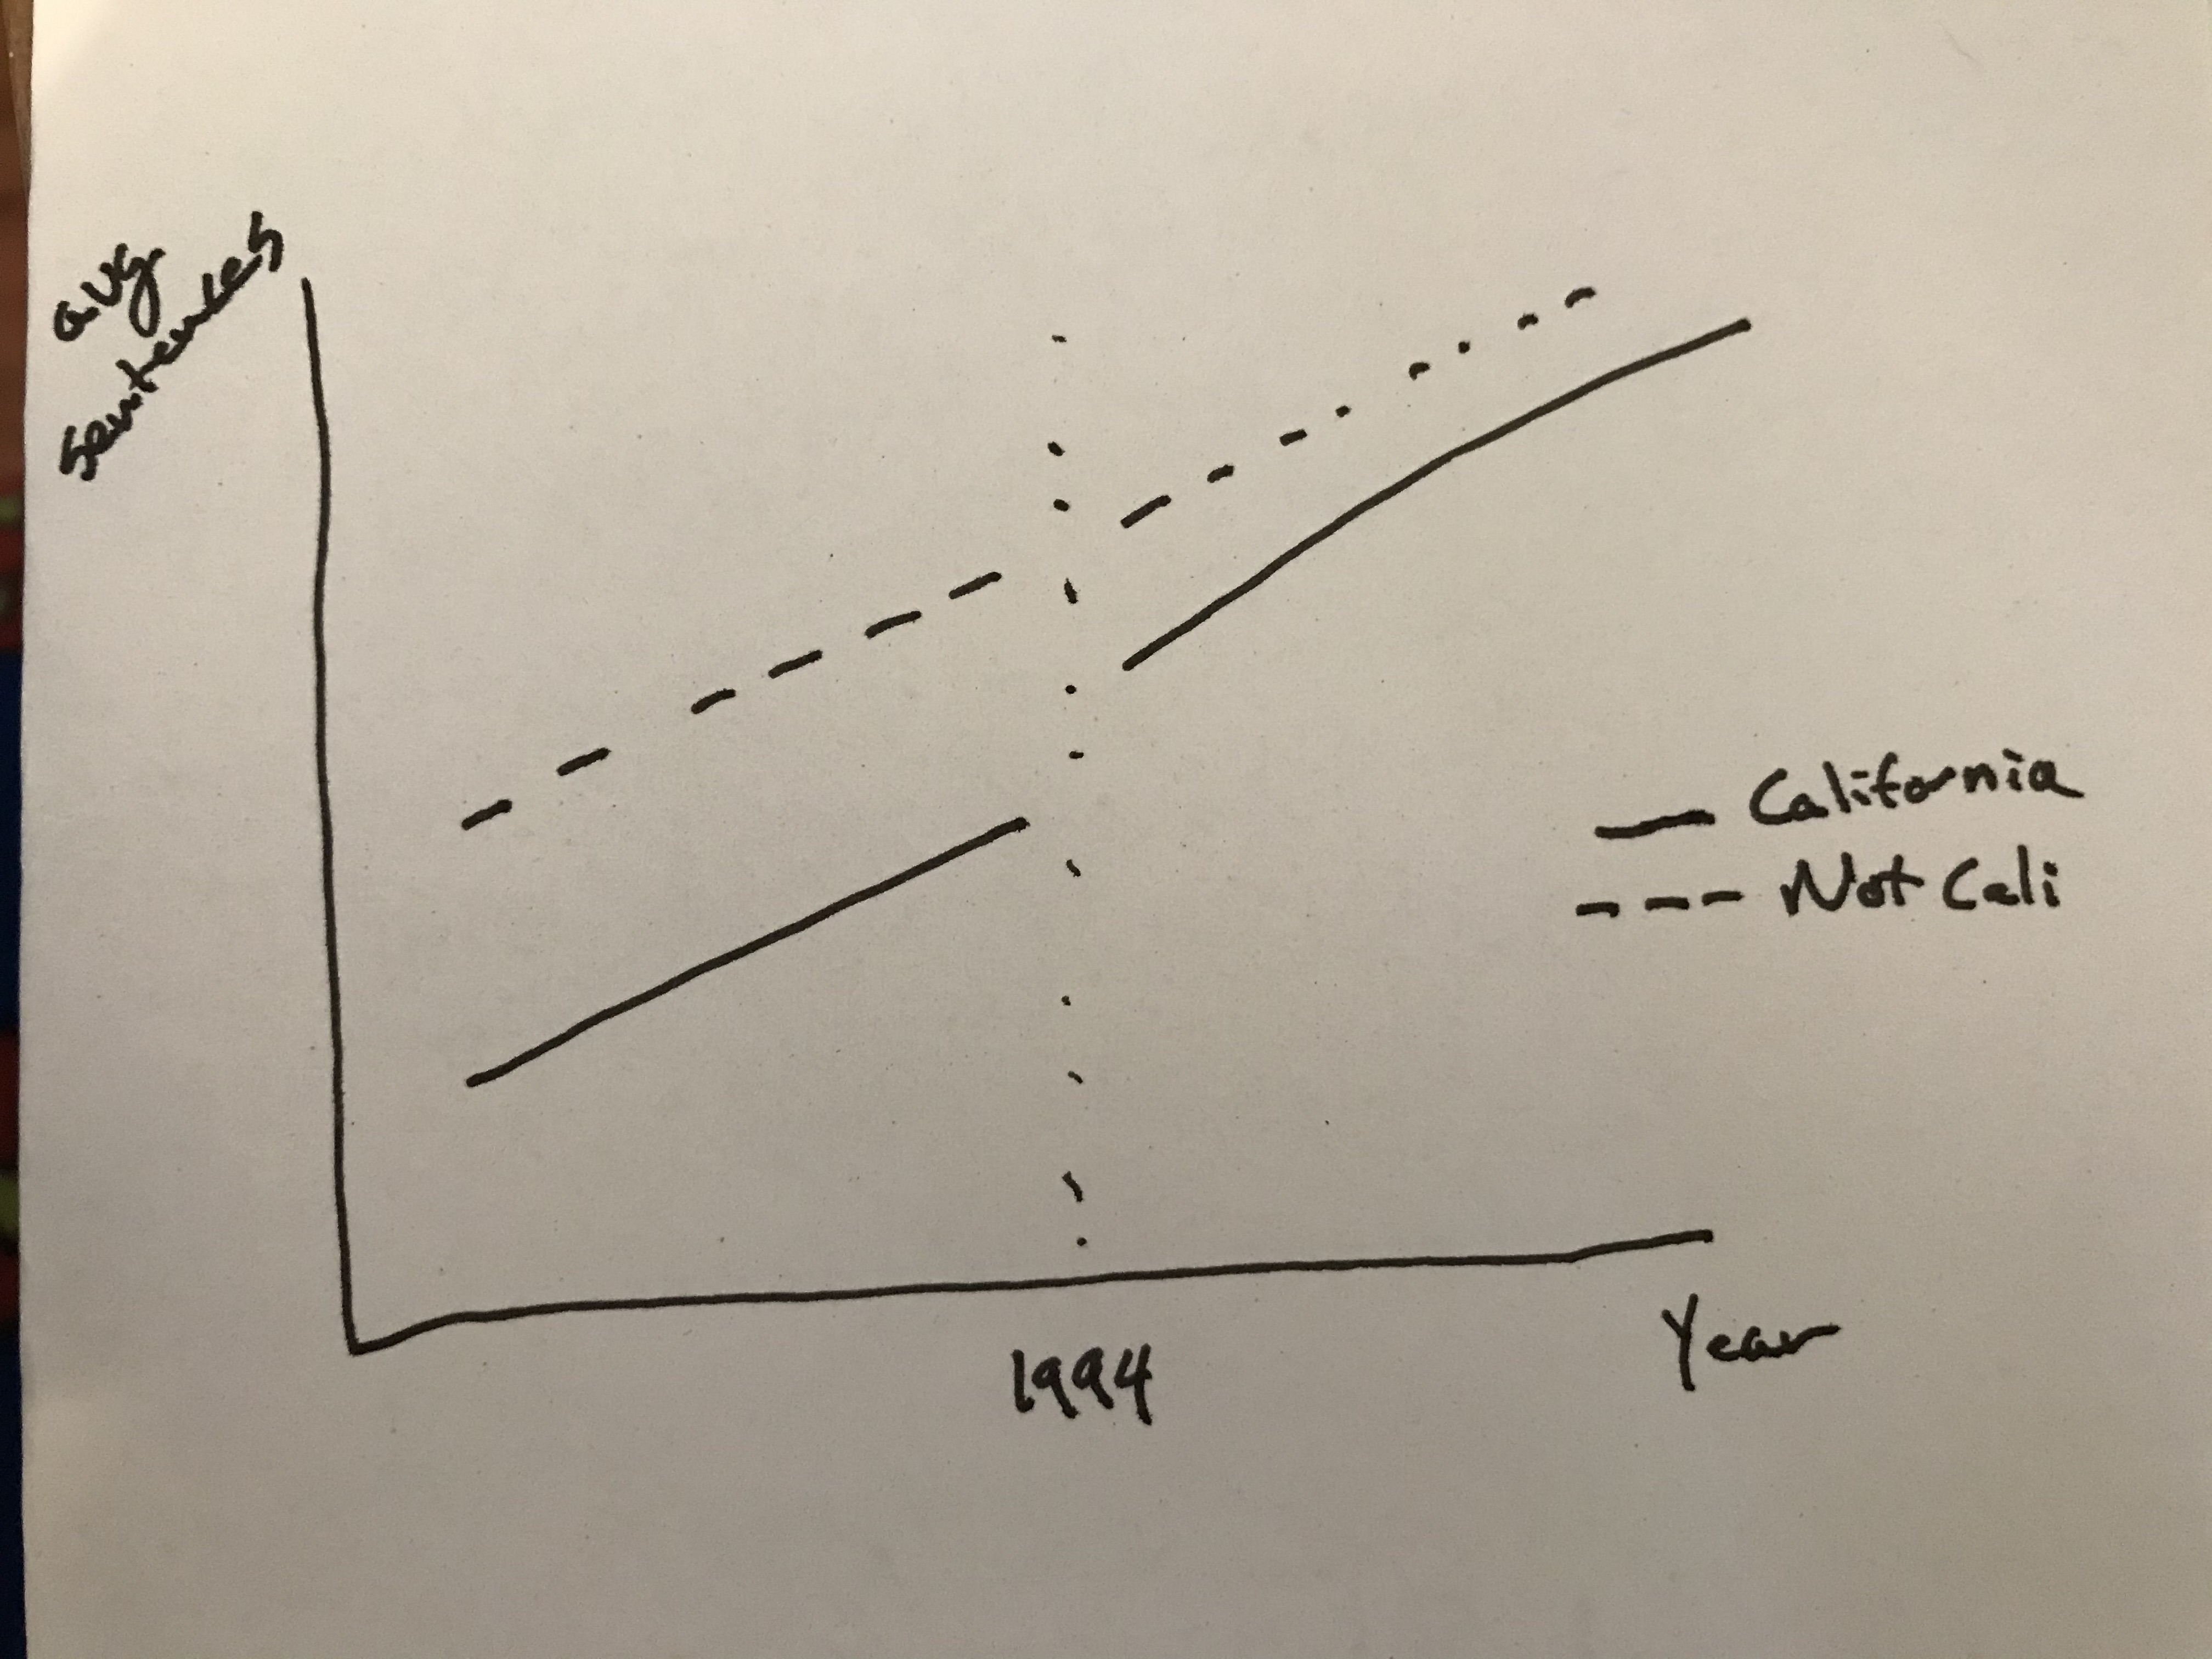
\includegraphics[width=\textwidth]{if_effect.jpg}
\end{figure}

\end{frame}


\begin{frame}[c]{}

\begin{figure}
    \centering
    \caption{If Doesn't Increase Incarceration}\label{}
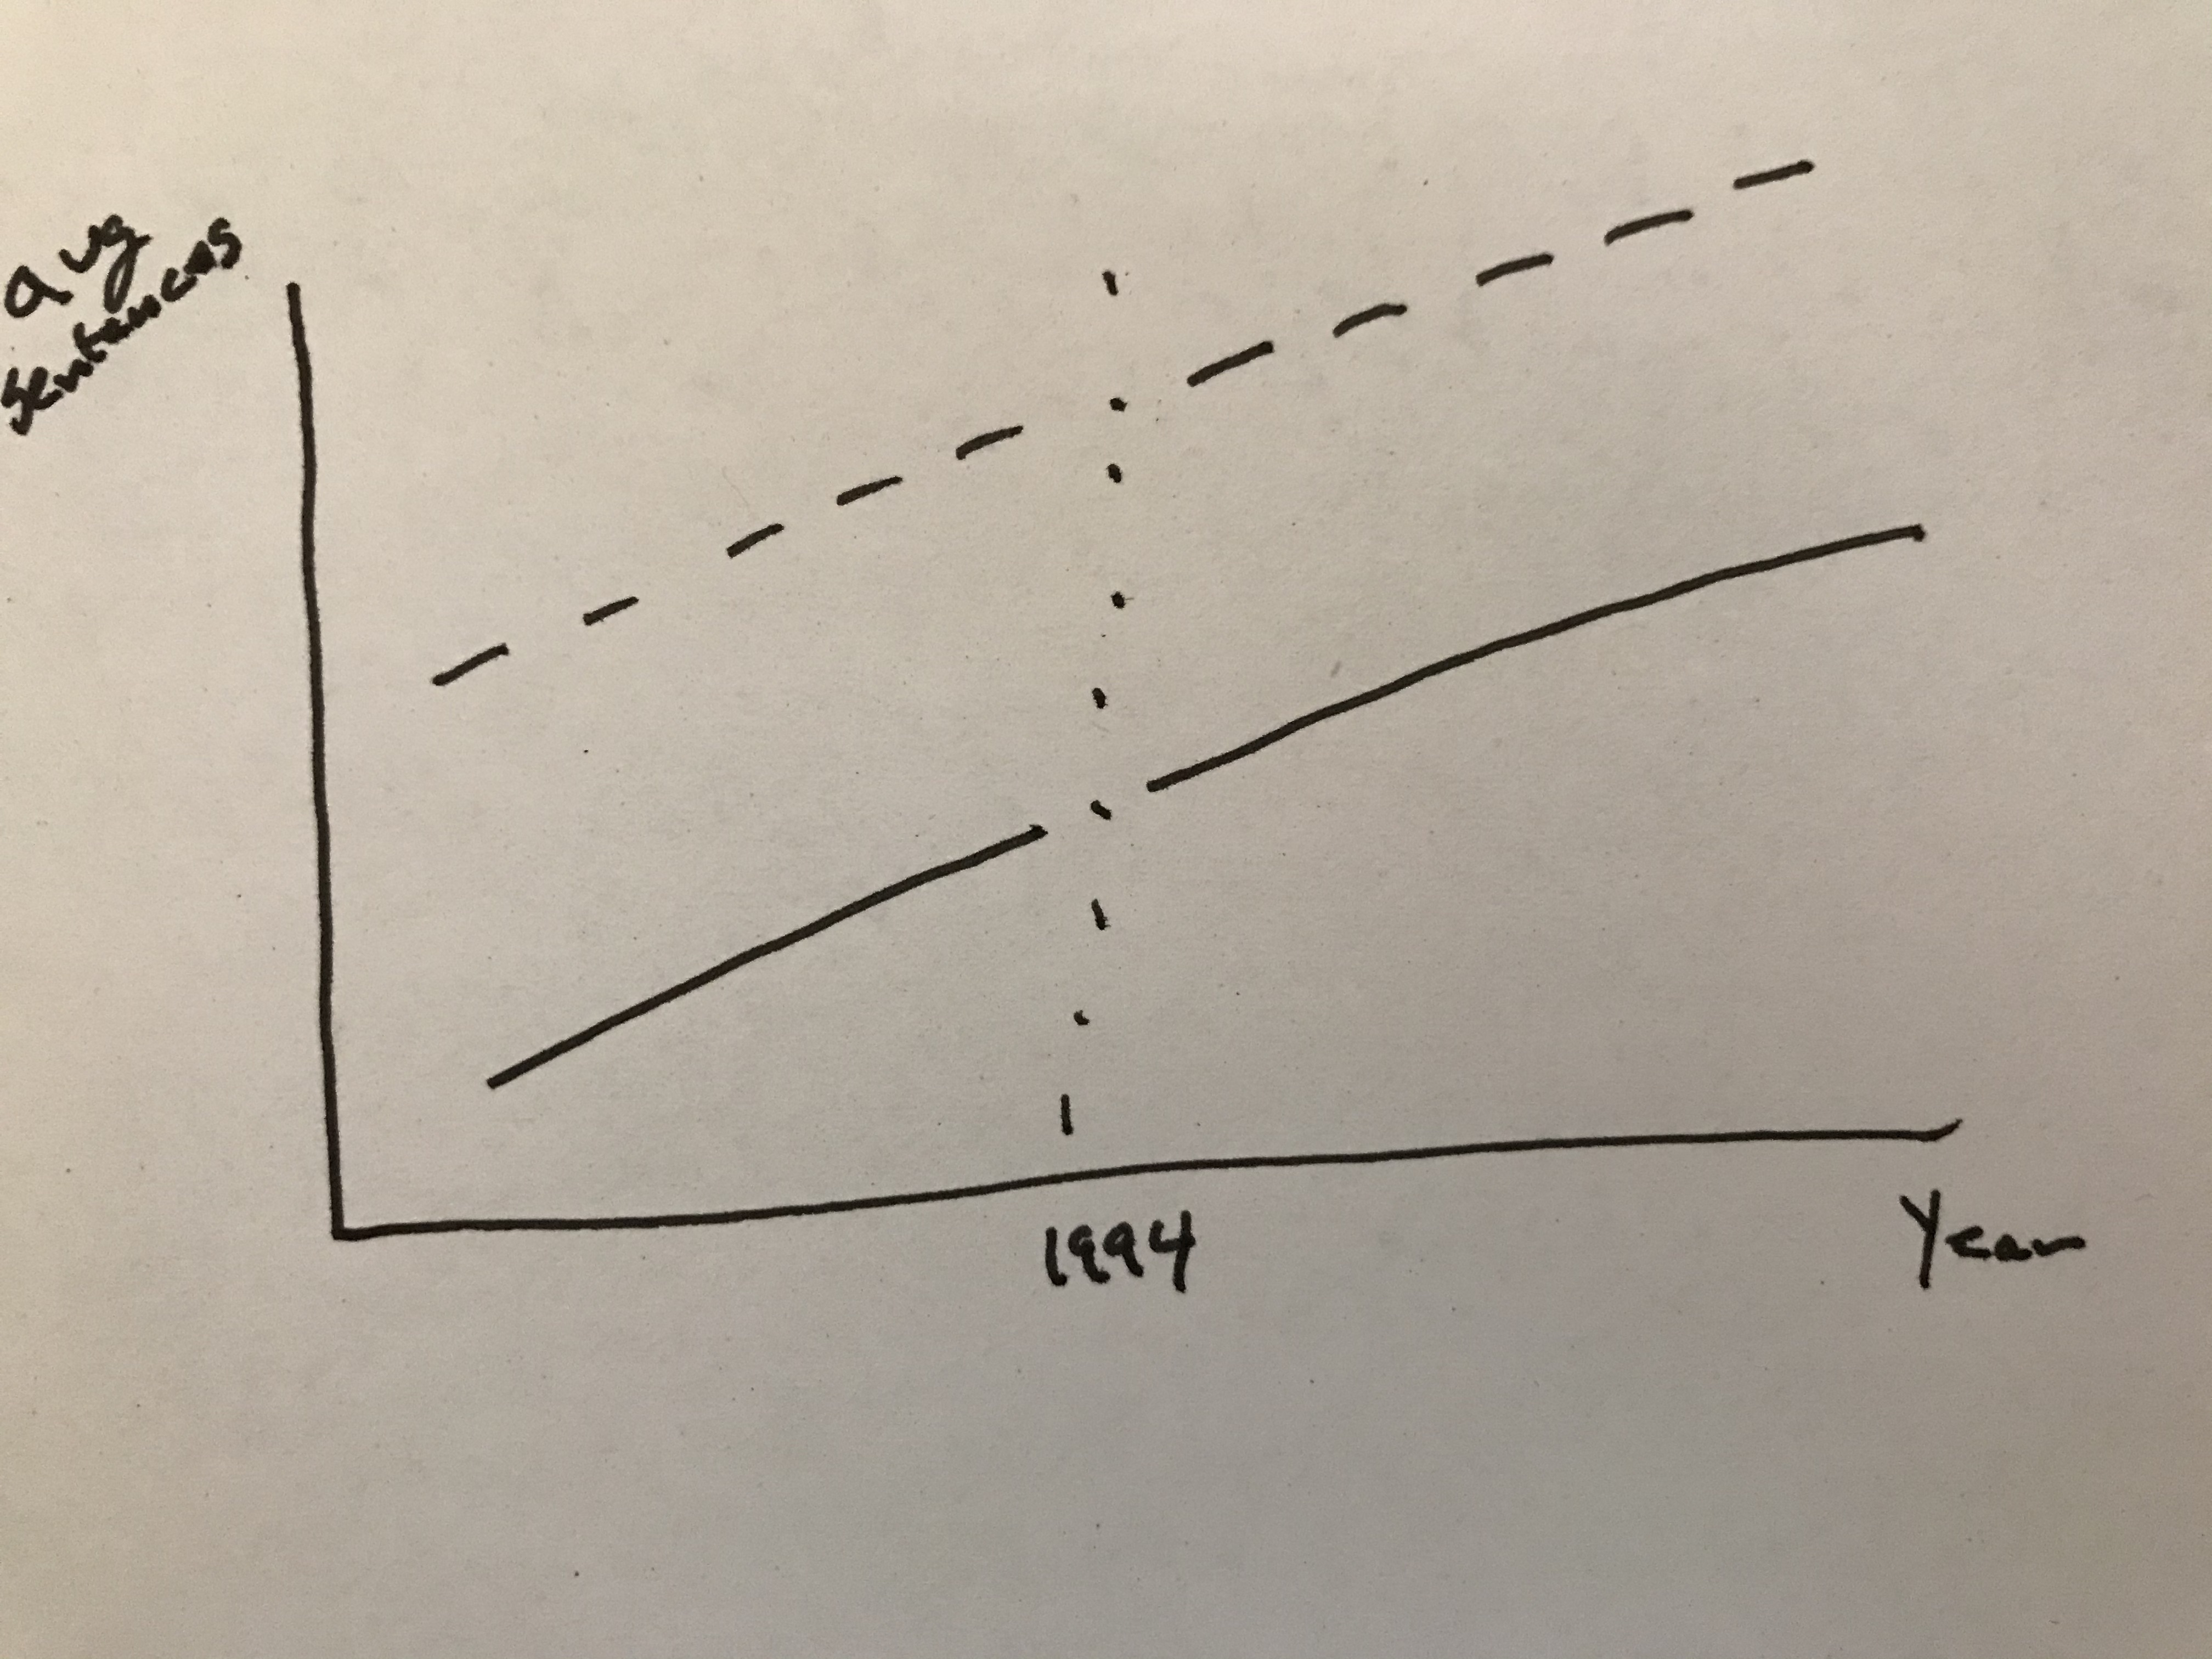
\includegraphics[width=\textwidth]{no_effect.jpg}
\end{figure}

\end{frame}


\begin{frame}[c]{Feasible Design \#2}
Many states in US passed changes in mandatory minimums between 1988 and late 1990s.
\pause \vspace{0.5cm}

Generalized Difference-in-Difference:
\begin{itemize}
    \item Compare states before and after passage of mandatory minimums,
    \item Controlling for common time trends.
\end{itemize}
Sample:
\begin{itemize}
    \item All US states.
\end{itemize}
\end{frame}


\begin{frame}[c]{Feasible Design \#2}
For state $s$ in year $t$:
\begin{eqnarray}
    PleaBargains_{s,t} &=& \boldsymbol{\alpha} + \boldsymbol{\beta_1} MandatoryMinimums_{s,t} + \boldsymbol{\beta_2} crime_{s,t} \nonumber \\
    && + \boldsymbol{\psi_{t}} + \boldsymbol{\gamma_{s}} + \epsilon_{s,t} \nonumber
\end{eqnarray}
Where:
\begin{itemize}
    \item $\psi_{t}$ are annual fixed effects
    \item $\gamma_{s}$ are state fixed effects
    \item $crime_{s,t}$ is crime rate in given state-year
\end{itemize}
\end{frame}

\begin{frame}[c]{Assumptions if Design \#2}
Absent mandatory minimum legislation, all states would have parallel trends in incarceration.
\end{frame}

\begin{frame}[c]{Data}
    \begin{itemize}
        \item \textbf{Mandatory minimum legislation:} in each state must be documented by searching news sources.
        \item \textbf{Plea Bargain Sentences} information comes from \emph{National Corrections Reporting Program}
        \item \textbf{Crime rates:} data comes from Uniform Crime Reporting database
    \end{itemize}
\end{frame}

\begin{frame}[c]{Recap}
    \alert{Does mandatory minimum legislation $\leadsto$ more punitive sentences?}
    \begin{itemize}
        \item Compare average sentences before and after passage of mandatory minimum legislation
        \pause \item Simple design: Western states before and after 1994 (Cali /not-Cali)
        \pause \item Generalized design: All US states, with timing of mandatory minimums varying by state
    \end{itemize}
    (Controlling for crime rates)
\end{frame}
\end{document}
